%-----------------------------------------------------------------
%	CAMP DE RADIACIÓ
%	!TEX root = ./../main.tex
%-----------------------------------------------------------------
\section{Camp de radiació}
\subsection{Conceptes bàsics}
La llum que rebem d'una estrella procedeix de la seva atmosfera, és a dir, de les capes superiors i transparents de gas que envolten l'interior (opac) de l'estrella. Aquí descriurem breument com viatja la llum a través de aquest gas.
\begin{figure}[h]
	\centering
	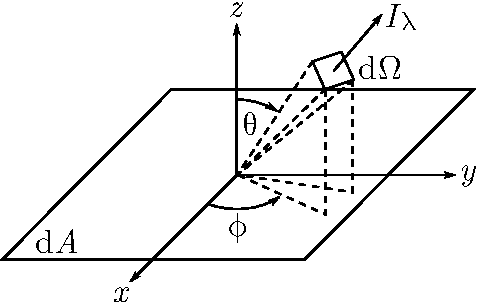
\includegraphics[width=0.4\textwidth]{./images/4-intensitat}
	\caption{Intensitat $I_{\lambda}$}
	\label{fig:intensitat}
\end{figure}

La figura \ref{fig:intensitat} mostra un raig de llum amb longitud d'ona entre $\lambda$ i $\lambda + \dd{\lambda}$ travesant una superfície $\dd{A}$ sota un angle $\theta$ respecte a la normal en un con d'angle sòlid $\dd{\Omega}$.

\subsubsection*{Intensitat}
\begin{defi}[Intensitat mitjana]
	Sigui $E_{\lambda}\dd{\lambda}$ l'energia que el raig porta a aquell con en un temps $\dd{t}$. Es defineix la intensitat mitjana d'aquest rang al quocient
	\begin{align}
	\bar{I}_{\lambda} = \frac{E_{\lambda} \dd{\lambda}}{\dd{\lambda} \dd{t} \dd{A} \cos \theta \dd{\Omega}}
	\end{align}
	Al CGS té unitats de $\qty[\bar{I}_{\lambda}] = \si{\erg \per \s \per \square\cm \per \steradian}$.
\end{defi}

\begin{defi}[Intensitat específica]
	En el límit $\dd{\Omega} \to 0$ el raig no es dispersa i la corresponent intensitat $I_{\lambda}$ es coneix com intensitat específica o simplement intensitat.
\end{defi}
En general la intensitat depèn de la direcció, de forma que la intensitat mitjana (sobre la direcció) s'escriu
\begin{align}
	\ev{I_{\lambda}} = \frac{1}{4\pi} \int I_{\lambda} \dd{\Omega} = \frac{1}{4\pi} \int_{\phi = 0}^{2\pi} \int_{\theta = 0}^{\pi} I_{\lambda} I_{\lambda} \sin \theta \dd{\theta} \dd{\phi}
\end{align}
Per a un camp isòtrop, $\ev{I_{\lambda}} \equiv I_{\lambda}$.

\subsubsection*{Energia}
\begin{defi}[Densitat d'energia]
	En un volum qualsevol (però que contingui moltes longituds d'ona), la densitat d'energia en l'interval $(\lambda, \lambda + \dd{\lambda})$ és
	\begin{align}
		u_{\lambda} \dd{\lambda} = \frac{1}{c} \int I_{\lambda} \dd{\lambda} \dd{\Omega} = \frac{4\pi}{c} \ev{I_{\lambda}} \dd{\lambda}
	\end{align}
\end{defi}
Per a un camp de radiació de cos negre (que és isòtrop), tenim que
\begin{align*}
	u_{\lambda} \dd{\lambda} = \frac{4\pi}{c} B_{\lambda} \dd{\lambda} = \frac{8\pi h c}{\lambda^{5}(e^{hc/\lambda k_{B} T} - 1)} \dd{\lambda}
\end{align*}
i en termes de la freqüència ($\nu = c/\lambda$), es pot reescriure com
\begin{align*}
	u_{\lambda} \dd{\nu} = \frac{4\pi}{c} B_{\nu} \dd{\nu} = \frac{8\pi h \nu}{\nu^{3}(e^{h \nu/k_{B} T} - 1)} \dd{\nu}
\end{align*}
Sumant totes les longituds d'ona, la densitat d'energia radiant d'un cos negre és
\begin{align}
	U = \int_{0}^{\infty} u_{\lambda} \dd{\lambda} = \frac{4\pi}{c} \int_{0}^{\infty} B_{\lambda}(T) \dd{\lambda} = \frac{4 \sigma}{c} T^{4} \equiv a T^{4}
\end{align}
on $a \equiv \dfrac{4\sigma}{c} = \SI{7.566}{\erg \per \cubic\cm \per \quartic\K}$ és la constant de radiació.

\begin{defi}[Flux radiant]
	$F_{\lambda} \dd{\lambda}$ és l'energia neta que amb longitud d'ona entre $\lambda$ i $\lambda + \dd{\lambda}$ passa a través de la unitat d'àrea en la unitat de temps per una direcció donada:
	\begin{align}
		F_{\lambda} \dd{\lambda} = \int I_{\lambda} \dd{\lambda} \cos \theta \dd{\Omega}
	\end{align}
	Al CGS té unitats de $\qty[F_{\lambda}] = \si{\erg \per \square\cm \per \s}$. Si el camp de radiació és isòtrop, llavors $F_{\lambda} = 0$.
\end{defi}

\subsubsection*{Pressió de radiació}
\begin{defi}
	Ja que cada fotó posseeix un moment lineal $p = E/c$, el camp de radiació associada té una pressió
	\begin{align}
		P_{rad,\lambda} \dd{\lambda} = \frac{2}{c} \int I_{\lambda} \dd{\lambda} \cos^{2} \theta \dd{\Omega}
	\end{align}
	Si el camp de radiació és de cos negre, integrant sobre $\lambda$ s'obté
	\begin{align}
		P_{rad} = \frac{4\pi}{3c} \int_{0}^{\infty} B_{\lambda}(T) \dd{\lambda} = \frac{1}{3} a T^{4} \equiv \frac{U}{3}
	\end{align}
\end{defi}

%-----------------------------------------------------------------
\subsection{Opacitat}
En travessar l'atmosfera estel·lar, la llum és en part absorbida (a unes longituds d'ona més que a altres), de manera que l'espectre que resulta no és exactament de cos negre.
\begin{figure}[H]
	\centering
	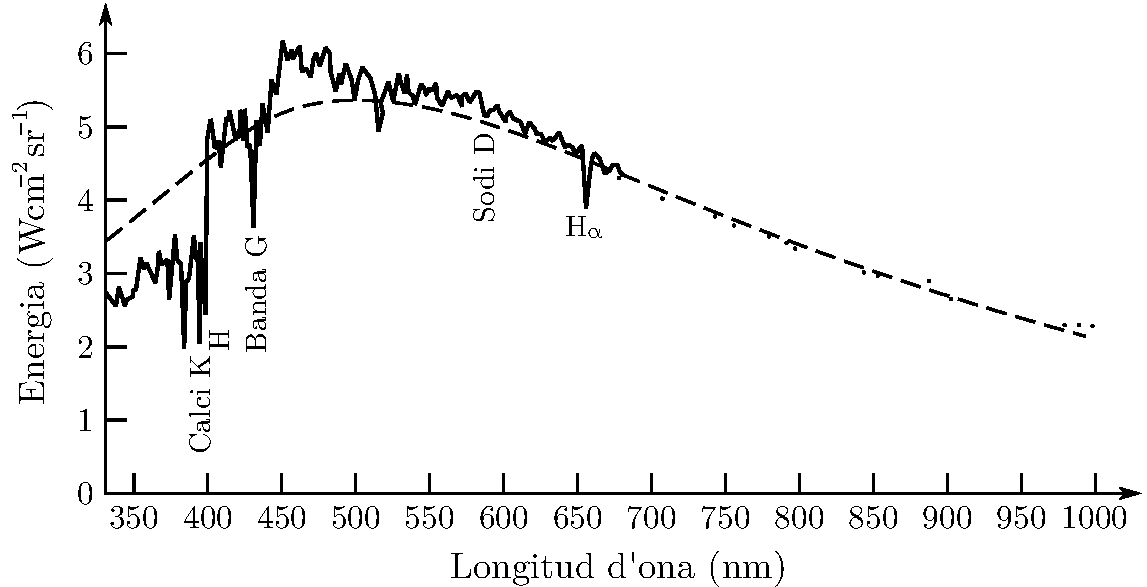
\includegraphics[width=0.8\textwidth]{./images/4-espectre-solar}
	\caption{Espectre solar}
	\label{fig:espectre-solar}
\end{figure}

La figura \ref{fig:espectre-solar} mostra l'espectre del Sol. La línia discontínua correspon a un cos negre de temperatura igual a la temperatura efectiva del Sol ($\SI{5770}{\K}$).

El decreixement de la intensitat a certes longituds d'ona es deu a l'absorció de la llum a aquestes longituds d'ona per metalls presents en l'atmosfera solar.

L'absorció es mesura mitjançant el \textit{coeficient d'absorció} o \textit{opacitat}, $\kappa_{\lambda}$.

Sigui un feix de llum, col·limat, que incideix sobre una placa de gas (figura \ref{fig:gas-opacitat}).
\begin{figure}[h]
	\centering
	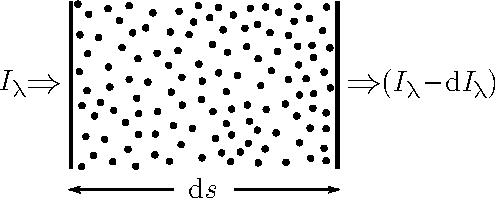
\includegraphics[width=0.45\textwidth]{./images/4-gas-opacitat}
	\caption{Placa de gas}
	\label{fig:gas-opacitat}
\end{figure}

La disminució d'intensitat al recórrer una distància $\dd{s}$ al gas de densitat $\rho$ és
\begin{align}\label{eq:int-opac}
	\dd{I}_{\lambda} = - \kappa_{\lambda} \rho I_{\lambda} \dd{s}
\end{align}
on $\kappa_{\lambda} > 0$ és la opacitat.

En general $\kappa_{\lambda}$ és una funció de la densitat del gas, la seva composició i temperatura. Al CGS té unitats de $\qty[\kappa_{\lambda}] = \si{\square\cm \per \g}$.

Convé advertir que en travesar el gas, es poden afegir fotons al feix per emissió dels àtoms de aquest gas. Així que l'equació \eqref{eq:int-opac} s'ha de generalitzar com
\begin{align}
	\dd{I}_{\lambda} = (j_{\lambda} - \kappa_{\lambda}) \rho I_{\lambda} \dd{s}
\end{align}
on $j_{\lambda}$ és el coeficient d'emissió del gas. De moment suposarem que $j_{\lambda} \equiv 0$.

Òbviament, si $\rho$ i $\kappa_{\lambda}$ són constants, l'equació \eqref{eq:int-opac} s'integra com
\begin{align}
	I_{\lambda}(s) = I_{\lambda 0} \exp[-\kappa_{\lambda} \rho s]
\end{align}

Així doncs, la distància típica que recorre un fotó qualsevol del feix abans d'abandonar-lo és
\begin{align*}
	l = \frac{1}{\kappa_{\lambda} \rho}
\end{align*}
aquesta és, a més a més, el \textit{recorregut lliure mig} dels fotons per procés de dispersió o \textit{scattering}.

\begin{example}
	En la fotosfera solar $\rho = \SI{2.5 e-7}{\g \per \cubic\cm}$, i la opacitat (per a $\lambda = \SI{5000}{\angstrom}$) $\kappa_{5000} = \SI{0.264}{\square\cm \per \g}$ , de manera que $l = \SI{1.52 e7}{\cm} = \SI{152}{\km}$.
\end{example}

%-----------------------------------------------------------------
\subsection{Profunditat òptica}
La profunditat òptica és un concepte unit estretament al d'opacitat. Quan observem la llum d'una estrella estem mirant al llarg del camí mitjà seguit pels fotons. Així doncs, es defineix profunditat òptica (\textit{optical depth}) com
\begin{align}\label{eq:opt-depth}
	\dd{\tau}_{\lambda} = - \kappa_{\lambda} \rho \dd{s}
\end{align}
on $s$ és la distància mesurada al llarg del camí del feix de llum en la direcció del moviment. Òbviament $\tau_{\lambda}$ és adimensional. Es pot veure que
\begin{align*}
	\Delta \tau_{\lambda} = \tau_{\lambda} - \tau_{\lambda 0} = - \int \kappa_{\lambda} \rho \dd{s}
\end{align*}
de manera que $\Delta \tau_{\lambda} < 0$.

Conforme la llum s'apropa a l'observador, aquesta viatja a través de valors més i més petits de $\tau_{\lambda}$. En les capes més externes de les estrelles $\tau_{\lambda} = 0$ ($\forall \lambda$). Així doncs,
\begin{align}
	\tau_{\lambda 0} = \int_{0}^{s} \kappa_{\lambda} \rho \dd{s}
\end{align}
és la profunditat òptica al llarg del raig en la seva posició inicial a la distància $s$ mesurada des de la superfície de l'atmosfera estel·lar.

Combinant \eqref{eq:int-opac} i \eqref{eq:opt-depth} i integrant s'obté
\begin{align}\label{eq:itau}
	I_{\lambda} = I_{\lambda 0} \exp[-\tau_{\lambda}]
\end{align}
de manera que la intensitat de llum decau exponencialment un cop abandona la superfície de l'estrella (sota la suposició que $\kappa_{\lambda}$ i $\rho$ són uniformes al llarg del camí seguit pel raig de llum).

Es pot veure que la profunditat òptica ens dóna el nombre de recorreguts lliures mitjos des de la superfície de l'estrella ($s > 0$) fins l'observador ($s = 0$):
\begin{align}
	l = \frac{1}{\kappa_{\lambda} \rho} \Rightarrow \tau_{\lambda} = \int_{0}^{s} \frac{\dd{s}}{l}
\end{align}
Ja que $\tau_{\lambda}$ depèn de $\lambda$, una atmosfera (o gas) pot ser òpticament gruixuda per a certes longituds d'ona i prima per a unes altres:
\begin{itemize}
	\item Si $\tau_{\lambda} \gg 1$, l'atmosfera es diu òpticament gruixuda (\textit{optically thick}).
	\item Si $\tau_{\lambda} \ll 1$, l'atmosfera es diu òpticament prima (\textit{optically thin}).
\end{itemize}

\begin{example}
	És obvi que les mesures del flux radioactiu rebut d'una estrella així com la magnitud aparent, $m$, han de ser corregides tenint en compte l'espessor de l'atmosfera terrestre.
	\begin{figure}[h]
		\centering
		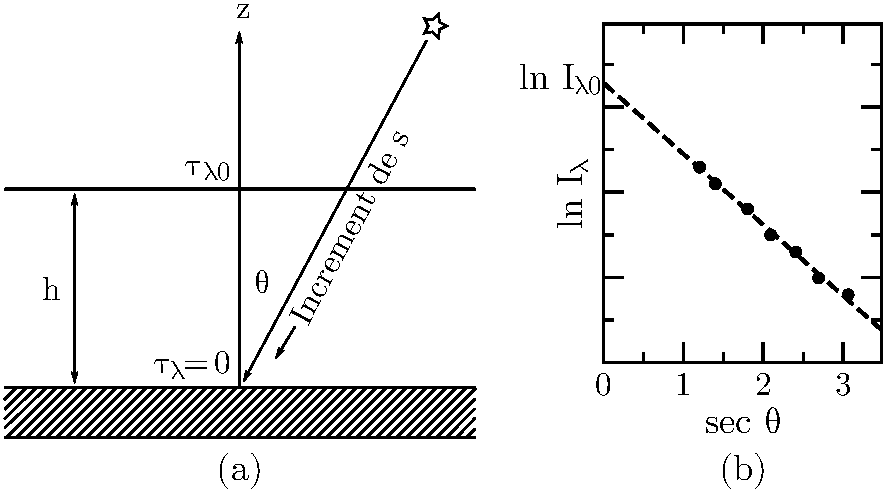
\includegraphics[width=0.6\textwidth]{./images/4-profunditat}
		\caption{(a) Un raig de llum entrant l'atmosfera terrestre amb un angle $\theta$, (b) $\ln I_{\lambda}$ en funció de $\sec \theta$}
		\label{fig:profunditat}
\end{figure}

	La figura \ref{fig:profunditat} mostra un raig que penetra en l'atmosfera terrestre sota un angle $\theta$ amb la vertical i viatjant fins un telescopi. L'alçada de l'atmosfera és $h$. La intensitat de la llum detectada al telescopi és $I_{\lambda}$.

	Es tracta de determinar $I_{\lambda 0}$. Per això considerem $\tau_{\lambda} = 0$ al telescopi (alçada zero), llavors
	\begin{align*}
		\tau_{\lambda} = \int_{0}^{s} \kappa_{\lambda} \rho \dd{s} = - \int_{0}^{h} \kappa_{\lambda} \rho \frac{\dd{z}}{\cos \theta} = \sec \theta \int_{0}^{h} \kappa_{\lambda} \rho \dd{z}
	\end{align*}
	Així doncs, $\tau_{\lambda} = \tau_{\lambda 0} \sec \theta$, de manera que
	\begin{align}
		I_{\lambda} = I_{\lambda 0} \exp[-\tau_{\lambda 0} \sec \theta]
	\end{align}
	però ens falta conèixer $I_{\lambda 0}$ i $\tau_{\lambda 0}$.

	Cap d'elles es pot determinar mitjançant una única observació. No obstant això, conforme la Terra gira en torn al seu eix, $\theta$ canvia, podent-se obtenir una gràfica (com a la figura \ref{fig:profunditat}) de $\ln I_{\lambda}$ en funció de $\sec \theta$.

	El pendent de la recta de regressió és $-\tau_{\lambda 0}$, i extrapolant la reca a $\sec \theta = 0$ s'obté gràficament $\ln I_{\lambda 0}$. Així es pot corregir la intensitat de flux radiant de l'absorció patida en travessar l'atmosfera terrestre.
\end{example}

%-----------------------------------------------------------------
\subsection{Fonts microscòpiques de l'opacitat}
Existeixen quatres processos principals que eliminen fotons d'un feix de llum mitjançant la interacció del fotó amb un electró (ja sigui aquest lliure o lligat, bé a un àtom neutre o a un ió):
\begin{figure}[h]
	\centering
	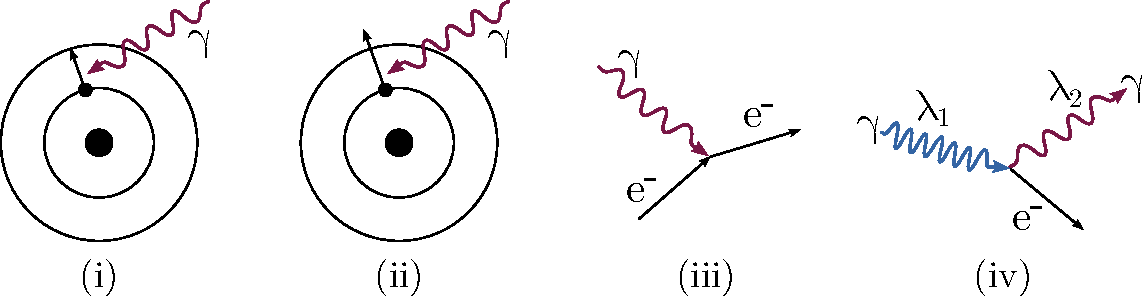
\includegraphics[width=0.8\textwidth]{./images/4-fonts-opacitat}
	\caption{(i) Transició lligat--lligat, (ii) transició lligat--lliure, (iii) absorció lliure--lliure, (iv) dispersió electrònica}
	\label{fig:fonts-opacitat}
\end{figure}

\begin{enumerate}[(i)]
	\item Transició lligat--lligat ($\kappa_{\lambda, bb}$): responsable de les ratlles d'absorció als espectres.
	\item Transició lligat--lliure ($\kappa_{\lambda, bf}$): font d'opacitat contínua, ja que pot eliminar del feix qualsevol fotó amb energia igual o superior a la d'ionització.
	\item Absorció lliure--lliure ($\kappa_{\lambda, ff}$): es tracta d'un procés de dispersió. Un electró lliure pròxim a un ió absorbeix un fotó i augmenta la seva velocitat. També contribueix a la opacitat contínua.

	El procés invers ($e^{-} \to e^{-} + \gamma$) rep el nom de \textit{Bremsstrahlung}.
	\item Dispersió electrònica ($\kappa_{es}$).
	\begin{enumerate}[(a)]
	\item Dispersió de Thomson: el fotó és dispersat per un electró lliure.

		És independent de $\lambda$ i és especialment eficaç a altes temperatures (la major part dels electrons són lliures a temperatures prou elevades). Aquest procés també contribueix a l'opacitat contínua.

		La secció eficaç de Thomson és
		\begin{align}
			\sigma_{T} = \frac{8\pi}{3} \qty(\frac{e^{2}}{m_{e} c^{2}}) = \SI{6.652 e-25}{\square\cm}
		\end{align}
		\item Dispersió de Compton: es dóna entre un fotó i un electró feblement lligat a un nucli atòmic si $\lambda \ll$ mida de l'àtom. També contribueix a l'opacitat contínua.
		\item Dispersió de Rayleigh: es dóna entre un fotó i un electró feblement lligat a un nucli atòmic si $\lambda \gg$ mida de l'àtom.

		La secció eficaç de Rayleigh és
		\begin{align}
			\sigma_{R} \propto \frac{1}{\lambda^{4}}
		\end{align}
		En la major part de les atmosferes estel·lars la dispersió de Rayleigh es pot menysprear. També contribueix a l'opacitat contínua.

		La dispersió de Rayleigh és responsable del color blau de la nostra atmosfera.
	\end{enumerate}
\end{enumerate}
És important senyalar que la font primària d'opacitat contínua en la majoria d'atmosferes estel·lars és la fotoionització d'ions \ch{H-} (un àtom format per $1p$ i $2e^{-}$). L'energia d'enllaç de l'electró addicional és $B = \SI{0.75}{\eV}$, de manera que qualsevol fotó amb $\lambda \leq hc/B = \SI{16400}{\angstrom}$ pot ser absorbit i l'electró alliberat.

Així doncs, aquest procés és una font important d'opacitat contínua des de la meitat de l'infraroig a longituds d'ona menors.

%-----------------------------------------------------------------
\subsection{Opacitat total}
L'opacitat total és la suma de totes les opacitats i depèn no només de la longitud d'ona sinó també de la composició, densitat i temperatura de l'atmosfera estel·lar:
\begin{align}
	\kappa_{\lambda} = \kappa_{\lambda, bb} + \kappa_{\lambda, bf} + \kappa_{\lambda, ff} + \kappa_{es}
\end{align}

\subsubsection*{Opacitat mitjana de Rosseland}
És l'opacitat obtinguda de fer la mitjana sobre $\lambda$, de manera que noés deoèn de la densitat, composició, i temperatura de l'atmosfera estel·lar. Així doncs, tenim $\bar{\kappa}_{\lambda, bb}$, $\bar{\kappa}_{\lambda, bf}$, $\bar{\kappa}_{\lambda, ff}$, i $\bar{\kappa}_{es}$.

L'opacitat total de Rosseland total és
\begin{align}
	\bar{\kappa} = \overline{\kappa_{\lambda, bb} + \kappa_{\lambda, bf} + \kappa_{\lambda, ff} + \kappa_{es}}
\end{align}
\begin{figure}[h]
	\centering
	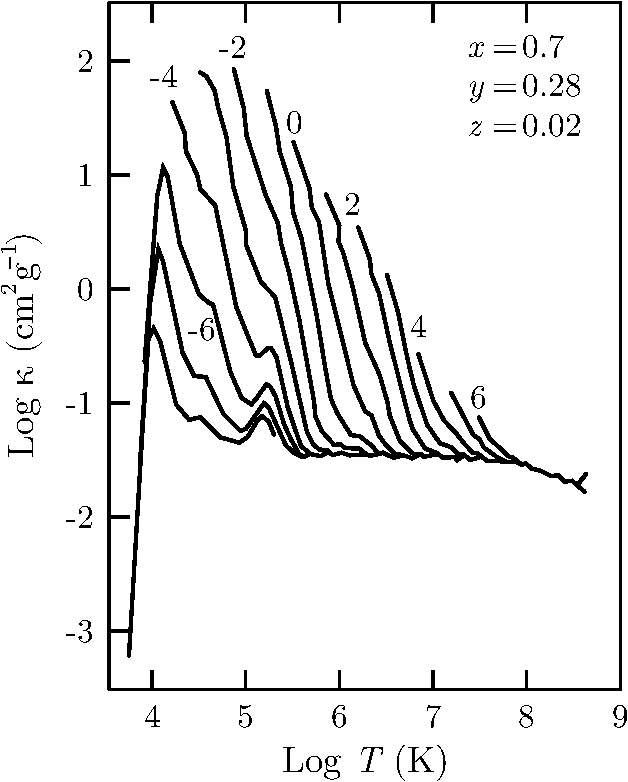
\includegraphics[width=0.45\textwidth]{./images/4-opacitat-rosseland}
	\caption{Opacitat mitjana de Rosseland. Les corbes estan etiquetades per $\log \rho$ en $\si{\g \per \cubic\cm}$}
	\label{fig:opacitat-rosseland}
\end{figure}

La figura \ref{fig:opacitat-rosseland} mostra $\bar{\kappa}$ en funció de la temperatura, amb $x = 0.7$, $y = 0.28$, $z = 0.02$ (on $x$, $y$, $z$ són les fraccions en pes d'hidrogen, heli i metalls, respectivament).

Inicialment $\bar{\kappa}$ creix quasi verticalment amb $T$ a causa del gran nombre d'electrons lliures procedents d'àtoms d'hidrogen i heli. Després d'assolir un màxim, les corbes cauen seguint aproximadament la llei de Kramers
\begin{align}
	\bar{\kappa} \propto T^{-3.5}
\end{align}
a causa de les absorcions lliure--lliure i lligat--lliure.

L'ió \ch{He} perd el seu únic electró aproximadament a $\SI{40000}{\K}$. Aquest lleuger augment d'electrons produeix el pic que s'observa en torn a aquesta temperatura.

En la zona inferior dreta de la figura, els gràfics posseeixen pendent nul. Allí domina l'absorció per dispersió d'electrons ja que a altes temperatures tots els electrons són lliures.
%-----------------------------------------------------------------
\subsection{Extinció}
La presència de pols i gas ocasiona que ens arribi menys llum de la que ens hauria arribat en absència d'aquests. Això, a més a més, provoca \textit{reddening}, l'empobriment de la llum en components  de curta longitud d'ona.

La quantificació sumultània d'ambdós efectes, ja que van units, es realitza mitjançant el paràmetre $A$. L'expressió $m - M = 5 \log(d/\SI{10}{\parsec})$ es converteix en
\begin{align}\label{eq:mMA}
	m - M = 5 \log(\frac{d}{\SI{10}{\parsec}}) + A
\end{align}
quan l'extinció (i/o reddening) es tenen en compte.

És obvi que si no hi hagués absorció (opacitat) es tindria $A = 0$ i la profunditat òptica seria $\tau = 0$.

\subsubsection*{Deducció de la relació entre $A$ i $\tau$}
Sigui $F_{0}$ el flux en la superfície d'una estrella de radi $R$, i $F(d)$ el seu valor a la distància $d$. Es pot veure que
\begin{align}\label{eq:iflux}
	I = \Omega F(d) d^{2} \Rightarrow I_{0} = \Omega F_{0} R^{2}
\end{align}
combinant \eqref{eq:itau} amb l'equació \eqref{eq:iflux} se segueix
\begin{align}
	F(d) = F_{0} \qty(\frac{R}{d})^{2} \exp[-\tau]
\end{align}
Per obtenir la distància mòdul, $m - M$, necessitem conèixer el flux que rebríem si l'estrella fos a $\SI{10}{\parsec} $ del nostre telescopi, avaluat sense extinció ($\tau = 0$):
\begin{align*}
	F(d) = F_{0} \frac{R^{2}}{(\SI{10}{\parsec})^{2}}
\end{align*}
La distància mòdul la podem escriure com
\begin{align*}
	m - M = -2.5 \log(\frac{F(d)}{F(\SI{10}{\parsec})}) = -2.5 \log[ \qty(\frac{\SI{10}{\parsec}}{d})^{2} \exp[-\tau]]
\end{align*}
és a dir
\begin{align}
	m - M = 5 \log(\frac{d}{\SI{10}{\parsec}}) + \qty(2.5 \log e) \tau
\end{align}
Comparant amb \eqref{eq:mMA}, obtenim
\begin{align}
	A_{\lambda} = \qty(2.5 \log e) \tau_{\lambda}
\end{align}
El subíndex $\lambda$ ens recorda que aquesta expressió és vàlida per a qualsevol longitud d'ona.

\begin{example}
	Cal trobar la profunditat òptica d'un banc de boira si el Sol vist a través d'aquest posseeix una lluminositat igual a la de la lluna plena en una nit perfecta. Dades: $m_{\odot} = -26.8$, $m_{L} = -12.5$.
	\begin{align*}
		A = m_{L} - m_{\odot} = \qty(2.5 \log e) \tau \Rightarrow \tau \approx 13.17
	\end{align*}
\end{example}

%-----------------------------------------------------------------
\subsection{Estructura de les línies espectrals}
La forma de la línia espectral conté una informació molt valuosa quant a l'ambient en què es va formar.
\begin{figure}[h]
	\centering
	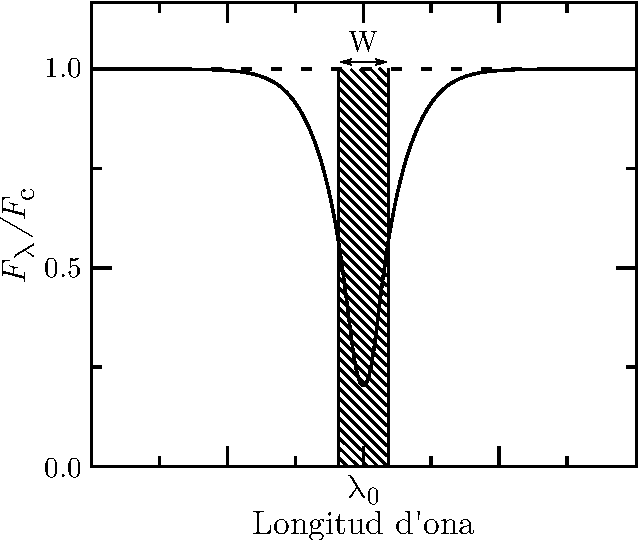
\includegraphics[width=0.5\textwidth]{./images/4-typical-spectral}
	\caption{Forma típica d'una línia espectral}
	\label{fig:typical-spectral}
\end{figure}

La figura \ref{fig:typical-spectral} mostra el flux radiant, $F_{\lambda}$, en funció de $\lambda$ per a una línia espectral típica.

La profunditat de la línia espectral és una funció de $\lambda$:
\begin{align}
	\frac{F_{c} - F_{\lambda}}{F_{c}}
\end{align}
on $F_{c}$ és el valor del flux radiant en l'espectre continu, i $\lambda_{0}$ la longitud d'ona al centre de la línia.

L'amplada de la línia (o amplada equivalent), $W$, sol ser $\approx \SI{0.1}{\angstrom}$:
\begin{align}
	W = \int \frac{F_{c} - F_{\lambda}}{F_{c}} \dd{\lambda}
\end{align}
Una altra mesura de l'amplada és l'amplada sencera a la meitat del màxim $(\Delta \lambda)_{1/2}$, és a dir, la distància de banda a banda de la línia espectral justament on se satisfà
\begin{align*}
	\frac{F_{c} - F_{\lambda}}{F_{c} - F_{\lambda 0}} = \frac{1}{2}
\end{align*}
En la figura \ref{fig:typical-spectral}, l'opacitat $\kappa_{\lambda}$ del material estel·lar és màxima en $\lambda_{0}$ (ja que allí l'absorció és màxima) i decreix conforme ens desplacem (a la dreta o esquerra de $\lambda_{0}$) pels costats de la línia espectral. Es pot concloure que el centre de la línia espectral (en $\lambda_{0}$) es va formar a les zones altes (i fredes) de l'atmosfera estel·lar. Conforme ens desplacem cap a dalt al llarg dels costats, aquests trams es van formar en zones més profundes i calents de l'atmosfera solar.

Hi ha tres efectes diferents que contribueixen a l'eixamplament de les línies espectrals.

\subsubsection*{Eixamplament natural}
Pel principi d'incertesa de Heisenberg, la incertesa en l'energia d'un electró en un orbital concret és
\begin{align*}
	\Delta E \approx \frac{\hbar}{\Delta t}
\end{align*}
on $\Delta t$ és l'interval de temps d'un electró en aquest orbital. Combinant aquesta equació amb
\begin{align*}
	E_{\gamma} = \frac{h c}{\lambda} \Rightarrow \dv{E}{\lambda} = - \frac{h c}{\lambda^{2}}
\end{align*}
arribem fàcilment a una expressió per l'eixamplament de les línies espectrals:
\begin{align}
	\Delta \lambda \approx \frac{\lambda^{2}}{2\pi c} \qty(\frac{1}{\Delta t_{i}} + \frac{1}{\Delta t_{f}})
\end{align}

\subsubsection*{Eixamplament per efecte Doppler}
En equilibri tèrmic, la velocitat més probable dels àtoms del gas és $v_{mp} = \sqrt{2 k_{B} T/m}$, i les longituds d'ona de la llum absorbida o emesa pels àtoms del gas seran desplaçades d'acord amb $\Delta \lambda / \lambda = \pm v_{r}/c$, de manera que
\begin{align}
	\Delta \lambda = \frac{2\lambda}{c} \sqrt{\frac{2 k_{B} T}{m}}
\end{align}
\begin{example}
	Per a àtoms d'hidrogen en la fotosfera solar ($T = \SI{5770}{\K}$) l'eixamplament per efecte Doppler de la línia $H_{\alpha}$ de l'hidrogen ($\lambda = \SI{6560.44}{\angstrom}$) resulta ser $\Delta \lambda = \SI{0.427}{\angstrom}$, aproximadament $\num{e3}$ vegades major que l'eixamplament natural.
\end{example}
Un estudi més detallat ens indica que l'eixamplament de la línia en la meitat del màxim és
\begin{align}
	(\Delta \lambda)_{1/2} = \frac{2\lambda}{c} \sqrt{\frac{2 k_{B} T}{m} \ln 2}
\end{align}
Si el moviment dels àtoms del gas és turbulent i la distribució de velocitats turbulentes segueix una distribució de Maxwell--Boltzmann, tenim
\begin{align}
	(\Delta \lambda)_{1/2} = \frac{2\lambda}{c} \sqrt{\qty[\frac{2 k_{B} T}{m} + v^{2}_{turb}] \ln 2}
\end{align}
Gràcies a aquest efecte es va poder inferir l'existència de fluxos turbulents en les atmosferes d'estrelles gegants i supergegants.

\subsubsection*{Eixamplament col·lisional i de pressió}
Col·lisions entre àtoms així com el camp elèctric d'un gran nombre d'ions passant a prop d'un àtom poden pertorbar els orbitals d'aquest.

Sense entrar en detalls de càlcul, es veu que l'eixamplament de les línies espectrals ve donat per
\begin{align}
	\Delta \lambda \approx \frac{\lambda^{2}}{c} \frac{n \sigma}{c} \sqrt{\frac{2 k_{B} T}{m}}
\end{align}
on $n$ és la densitat numèrica d'àtoms, i $\sigma$ és la secció eficaç de col·lisió.
\begin{example}
	Per a àtoms d'hidrogen en la fotosfera solar ($T = \SI{5770}{\K}$) l'eixamplament col·lisional i de pressió de la línia $H_{\alpha}$ de l'hidrogen ($\lambda = \SI{6560.44}{\angstrom}$) resulta ser $\Delta \lambda = \SI{2.36 e-4}{\angstrom}$, valor similar a l'eixamplament natural.
\end{example}
